\documentclass[a4paper,10pt]{article}

\usepackage{graphicx}
\usepackage{amsmath}
\usepackage[spanish]{babel}
\usepackage[utf8]{inputenc} % Permite escribir directamente áéíóúñ
\usepackage{float}
\usepackage[hidelinks]{hyperref}
\usepackage{pdfpages}
\usepackage{multirow}
\usepackage[margin=0.9in]{geometry}

\title{ \textbf{ 7529. Teoría de Algoritmos I\\
Trabajo Práctico 1}}

\author{ Hall, Laura, \textit{Padrón Nro. 94237} \\
\texttt{ laurahall@ymail.com } \\[2.5ex]
Martin, Débora, \textit{Padrón Nro. 90934} \\
\texttt{ demartin@fi.uba.ar } \\[2.5ex]
\normalsize{2do. Cuatrimestre de 2016} \\
}

\date{}

\begin{document}
\maketitle
\thispagestyle{empty} % quita el nmero en la primer pagina
\setcounter{page}{0}
\newpage
\tableofcontents

\newpage

\section{Estadístico de orden k}

Consideraremos en todos los casos que el número de elementos del conjunto considerado es n.

\subsection{Fuerza bruta}

El algoritmo de fuerza bruta recorre los elementos del arreglo, y a cada uno lo compara contra todos los demás para determinar la cantidad de elementos menores al considerado. Si encuentra alguno para el cual dicha cantidad sea k, corta el ciclo en ese momento y lo devuelve como resultado. 

\begin{itemize}

\item \textbf{Complejidad:} $O(n^2)$
\item \textbf{Mejores casos:}
	\begin{itemize}
	\item $O(n)$ si el elemento con k menores se encuentra en la primera posición. Ej:
	\begin{verbatim}
	conjunto = {0, 6, 3, 7, 10, 11, 15, 8, 2, 4, 13, 1, 5, 12, 9, 14}
	\end{verbatim}
	\end{itemize}

\item \textbf{Peores casos:}
	\begin{itemize}
	\item $O(n^2)$ si el elemento con k menores se encuentra en la última posición. Ej:
	\begin{verbatim}
	conjunto = {14, 6, 3, 7, 10, 11, 15, 8, 2, 4, 13, 1, 5, 12, 9, 0}
	\end{verbatim}
	\end{itemize}

\end{itemize}
	

\subsection{Ordenar y seleccionar}

Este algoritmo tiene dos partes. La primera, que ordena el conjunto por el método de quicksort, y la segunda, que selecciona un elemento de ese conjunto. Esta última parte se efectúa en tiempo constante, por lo que el orden del algoritmo dependerá completamente del orden de quicksort. Dicho algoritmo depende fuertemente de la elección del pivote, pero en un caso promedio es $O(n \log{n})$.

\begin{itemize}

\item \textbf{Complejidad:} $O(n \log{n})$
\item \textbf{Mejores casos:}
	\begin{itemize}
	\item $O(n \log{n})$ si el pivote, luego de ordenado el conjunto, se halla en una posición central del mismo. Es decir, hay igual cantidad de elementos menores y mayores al pivote. Ej:
	\begin{verbatim}
	conjunto = {0, 6, 3, 7, 10, 11, 15, 8, 2, 4, 13, 1, 5, 12, 9, 14}
	pivote = 8
	\end{verbatim}
	\end{itemize}
\item \textbf{Peores casos:}
	\begin{itemize}
	\item $O(n^2)$ si la mayoría de los elementos son menores que el pivote. Ej:
	\begin{verbatim}
	conjunto = {0, 6, 3, 7, 10, 11, 15, 8, 2, 4, 13, 1, 5, 12, 9, 14}
	pivote = 14
	\end{verbatim}
	\item $O(n^2)$ si la mayoría de los elementos son mayores que el pivote. Ej:
	\begin{verbatim}
	conjunto = {0, 6, 3, 7, 10, 11, 15, 8, 2, 4, 13, 1, 5, 12, 9, 14}
	pivote = 0
	\end{verbatim}
	\end{itemize}

\end{itemize}

\subsection{K-selecciones}

El ordenamiento por selección es $O(n^2)$ porque recorre todo el conjunto para hallar el menor, lo coloca en el primer lugar y vuelve a repetir el proceso para todos los elementos restantes. Dado que no pretendemos ordenar todo el arreglo, sino solo encontrar el k-ésimo elemento menor, deberemos recorrer el conjunto de tamaño n, $k+1$ veces. Es decir, si k es cero, se recorre una vez.

\begin{itemize}

\item \textbf{Complejidad:} $O(n*(k+1))$
\item \textbf{Mejores casos:}
	\begin{itemize}
	\item $O(n)$ si k es cero. Ej:
	\begin{verbatim}
	k = 0
	conjunto = {14, 6, 3, 7, 10, 11, 15, 8, 2, 4, 13, 1, 5, 12, 9, 0}
	\end{verbatim}
	\end{itemize}
\item \textbf{Peores casos:}
	\begin{itemize}
	\item $O(n^2)$ si k es igual a $n-1$.
	\begin{verbatim}
	k = 15
	conjunto = {15, 6, 3, 7, 10, 11, 0, 8, 2, 4, 13, 1, 5, 12, 9, 14}
	\end{verbatim}
	\end{itemize}
	
\end{itemize}

\subsection{K-heapsort}

El heapsort tiene una complejidad de $O(n \log{n})$. Ya que extraer un elemento de este obliga a realizar un downheap, cada extracción será $O(\log n)$. Si se realizan k extracciones, se deberá realizar un downheap k veces. Acceder al elemento en la raiz se realiza en orden constante. Por lo tanto la complejidad del K-Heapsort será $O(n \log{n} + k \log{n})$. Como k puede ser a lo sumo igual a $n-1$, el orden del algoritmo será como máximo $O(2n \log{n})$, es decir $O(n \log{n})$.

\begin{itemize}

\item \textbf{Complejidad:} $O(n \log{n})$
\item \textbf{Mejores casos:}
	\begin{itemize}
	\item $O(n \log{n})$ si k es igual a cero. Porque solo debo realizar el ordenamiento de heapsort y evito los downheap de cada extracción. Ej:
	\begin{verbatim}
	k = 0
	conjunto = {15, 6, 3, 7, 10, 11, 0, 8, 2, 4, 13, 1, 5, 12, 9, 14}
	minheap = {0, 2, 1, 7, 4, 3, 6, 14, 8, 10, 13, 11, 5, 12, 9, 15}
	\end{verbatim}
	
	\end{itemize}
\item \textbf{Peores casos:}
	\begin{itemize}
	\item $O(2n \log{n})$ si k es igual a $n-1$. Ej:
	\begin{verbatim}
	k = 0
	conjunto = {15, 6, 3, 7, 10, 11, 0, 8, 2, 4, 13, 1, 5, 12, 9, 14}
	minheap = {0, 2, 1, 7, 4, 3, 6, 14, 8, 10, 13, 11, 5, 12, 9, 15}
	minheap.pop()
	minheap = {1, 2, 3, 7, 4, 5, 6, 14, 8, 10, 13, 11, 15, 12, 9}
	minheap.pop()
	minheap = {2, 4, 3, 7, 9, 5, 6, 14, 8, 10, 13, 11, 15, 12}
	...
	\end{verbatim}
	\end{itemize}
\end{itemize}

\subsection{HeapSelect}

HeapSelect usa un heap de máximo, pero este heap tiene un total de k elementos. Esto implica que las operaciones, como la de remover la raiz, serán $O(\log{k})$. Para determinar los menores elementos se comparan todos contra el máximo del heap. En caso de que alguno sea menor que el máximo, se lo agrega al heap, removiendo el máximo anterior. Esto implicará dos operaciones $O(\log{k})$.

\begin{itemize}
\item \textbf{Complejidad:} $O(n \log{k})$
\item \textbf{Mejores casos:}
	\begin{itemize}
	\item $O(k \log{k})$ si los $k+1$ elementos menores están en las primeras posiciones del conjunto, lo que evita modificar el heap luego de su creación. Ej:
	\begin{verbatim}
	k = 4
	conjunto = {1, 0, 3, 2, 4, 11, 6, 8, 7, 10, 13, 15, 5, 12, 9, 14}
	maxheap = {4,2,3,1,0}
	\end{verbatim}
	\end{itemize}
\item \textbf{Peores casos:}
	\begin{itemize}
	\item $O(n \log{k})$ si los $k+1$ elementos menores están en las últimas posiciones del conjunto, lo que evita que implica que todos los elementos del conjunto serán agregados al heap y la $n-k$ serán removidos. Ej:
	\begin{verbatim}
	k = 4
	conjunto = {11, 6, 8, 7, 10, 13, 15, 5, 12, 9, 14, 1, 0, 3, 2, 4}
	\end{verbatim}
	\end{itemize}
\end{itemize}

\subsection{QuickSelect}

La complejidad de QuickSelect depende en buena medida de la elección del pivote debido a que este determina que cantidad de elementos serán descartados en el siguiente paso de la búsqueda. En caso de elegir un pivote que descarte pocos elementos, la cantidad de pasos será mayor. A diferencia de Quicksort, no busca sobre todos los elementos en los sucesivos pasos, sino que solo busca sobre el segmento que contiene al elemento objetivo.

\begin{itemize}
\item \textbf{Mejores casos:}
	\begin{itemize}
	\item $O(n)$ si el pivote coincide con el elemento buscado. En tal caso solo realiza una partición del conjunto que requiere leer todo una vez. Ej:
	\begin{verbatim}
	k = 4
	indicePivote = (n-1)/2
	conjunto = {11, 6, 8, 7, 10, 13, 15, 4, 12, 9, 14, 1, 0, 3, 2, 5}
	conjuntoDespuesQuickSelect = {1, 0, 3, 2, 4, 13, 15, 5, 12, 9, 14, 11, 6, 8, 7, 10}
	\end{verbatim}
	\end{itemize}
\item \textbf{Peores casos:}
	\begin{itemize}
	\item $O(n^2)$ si el conjunto está ordenado. Va quitando elementos del conjunto de a uno, lo que implica realizar $n-1$ particiones. Ej:
	\begin{verbatim}
	k = 4
	indicePivote = (n-1)
	conjunto = {0, 1, 2, 3, 4, 5, 6, 7, 8, 9, 10, 11, 12, 13, 14, 15}
	conjuntoPrimerParticion = {0, 1, 2, 3, 4, 5, 6, 7, 8, 9, 10, 11, 12, 13, 14}
	\end{verbatim}
	\end{itemize}
\end{itemize}


\subsection{Tiempos de ejecución}

Se realizó un muestreo de los tiempos de ejecución de los distintos algoritmos. Para ello se usaron tres conjuntos de 10000 elementos aleatorios. Se tomaron los tiempos para cada uno y se obtuvo un promedio de los mismos. Para k se usaron 6 valores distintos.

\begin{figure}[H]
\begin{center}
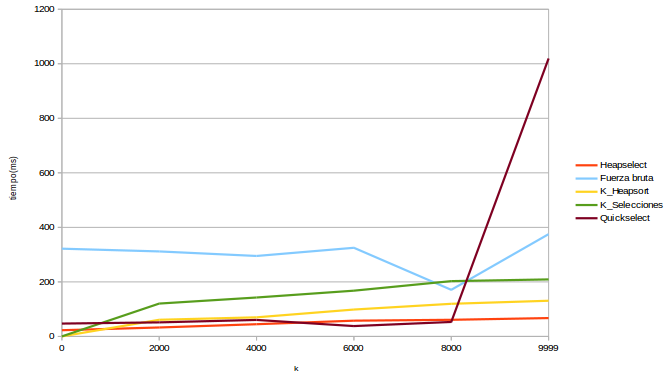
\includegraphics[width=0.8\textwidth]{./tiempoSegunK.png}
\label{fig:tiempos}
\caption{Tiempos de ejecución de los algoritmos en función de k}
\end{center}
\end{figure}

Del anterior gráfico se puede concluir claramente que, en promedio, fuerza bruta es el que peor se comporta para la mayoría de los k. Según lo predicho, K\_Heapsort y K\_Selecciones tienen su mejor caso en k igual a cero. QuickSelect tiene un excelente desempeño en el promedio de los k, sin embargo tiene algunos casos problemáticos que, si bien no dependen directamente del valor de k, sí deben ser tenidos en cuenta. En particular hay que notar que la elección del pivote fue absolutamente arbitraria. HeapSelect, tiene un muy buen desempeño. Es mucho más constante, practicamente invariante con respecto a k. 

\section{Recorridos en grafos}

En todos los casos consideraremos grafos en los cuales los vértices origen y destino pertenezcan a la misma componente conexa de modo que exista un camino entre ellos.

\subsection{BFS}

El recorrido en anchura explora el grafo por niveles pasando por todos sus vertices y aristas. Es decir, su complejidad es $O(|V| + |A|)$ siendo $|V|$ la cantidad de vertices del grafo y $|A|$ la cantidad de aristas. El algoritmo implementado corta la ejecución en caso de encontrar el vértice destino.

\begin{itemize}
\item \textbf{Complejidad:} $O(|V| + |A|)$
\item \textbf{Mejores casos:}
	\begin{itemize}
	\item $O(1)$ en el caso trivial en que el vertice origen es igual al vertice destino.
	\item $O(|V_m| + |A_m|)$ siendo $|V_m|$ la cantidad de vertices pertenecientes al camino mínimo y $|A_m|$ la cantidad de aristas cuando el grafo es lineal. Ej:
	\begin{verbatim}
	origen = 1
	destino = 5
	\end{verbatim}
	\begin{figure}[H]
	\begin{center}
	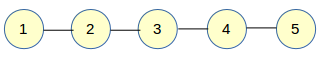
\includegraphics[width=0.3\textwidth]{./g1.png}
	\label{fig:g1}
	\end{center}
	\end{figure}
	\item $O(|V_n| + |A_n|)$ con $|V_n|$ la cantidad de vertices en niveles menores o iguales a $n$ y $|A_n|$ la cantidad de aristas correspondientes, si el primer camino evaluado es el camino mínimo. En el ejemplo se muestran dos caminos, pero solo hay uno mínimo (rojo) y será el primero que se considerará. Ej:
	\begin{verbatim}
	origen = 1
	destino = 5
	\end{verbatim}
	\begin{figure}[H]
	\begin{center}
	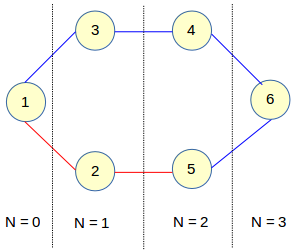
\includegraphics[width=0.3\textwidth]{./g2.png}
	\label{fig:g2}
	\end{center}
	\end{figure}
	\end{itemize}

\item \textbf{Peores casos:}
	\begin{itemize}
	\item $O(|V| + |A|)$ si el destino es el último vertice en ser evaluado por estar en el mayor nivel posible. Ej:
	\begin{verbatim}
	origen = 1
	destino = 6
	\end{verbatim}
	\begin{figure}[H]
	\begin{center}
	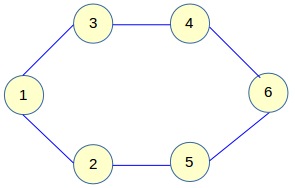
\includegraphics[width=0.3\textwidth]{./g3.png}
	\caption{Grafo no ponderado 1}
	\label{fig:g3}
	\end{center}
	\end{figure}
	\item Si el grafo es ponderado puede no escoger el camino mínimo. En el ejemplo, el camino en rojo sería el elegido, a pesar de existir uno mejor. Ej:
	\begin{verbatim}
	origen = 1
	destino = 6
	\end{verbatim}
	\begin{figure}[H]
	\begin{center}
	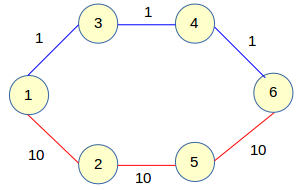
\includegraphics[width=0.3\textwidth]{./g4.png}
	\caption{Grafo ponderado 1}
	\label{fig:g4}
	\end{center}
	\end{figure}
	\end{itemize}
\end{itemize}

\subsection{Dijkstra}

Para implementar este algoritmo se usó una cola de prioridad. Por lo tanto, la complejidad estará dada en buena medida por el costo de las operaciones de dicha estructura, que son $O(n \log{n})$. En particular, en cada paso se elimina un vertice de la cola($O(|V| \log{|V})$), se analiza si sus adyacentes están visitados y en caso contrario se los agrega a la cola($O(|A| \log{|V|})$). Es decir, se realizan $O((|A| + |V|) \log{|V|})$. Esto es equivalente a $O(|A| \log{|V|})$. Al ser tan similar a BFS, los mejores y pe

\begin{itemize}
\item \textbf{Complejidad:} $O(|A| \log{|V|})$
\item \textbf{Mejores casos:}
	\begin{itemize}
	\item $O(|V| \log{|V|})$ si la primer distancia asignada a cada vertice es la mínima al origen de modo que no sea necesario agregar y quitar el mismo vertice repetidas veces de la cola. Ej:
	\begin{verbatim}
	origen = 1
	destino = 4
	\end{verbatim}
	\begin{figure}[H]
	\begin{center}
	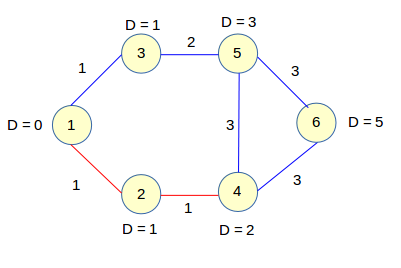
\includegraphics[width=0.4\textwidth]{./g5.png}
	\caption{Grafo ponderado 2}
	\label{fig:g5}
	\end{center}
	\end{figure}
	\end{itemize}
\item \textbf{Peores casos:}
	\begin{itemize}
	\item $O(|A| \log{|V|})$ si es necesario agregar y quitar los mismos vertices repetidas veces de la cola por haber actualizado su distancia. En el ejemplo esto sucede con los vértices 2, 4, 5 y 6. Ej:
	\begin{verbatim}
	origen = 1
	destino = 6
	\end{verbatim}
	\begin{figure}[H]
	\begin{center}
	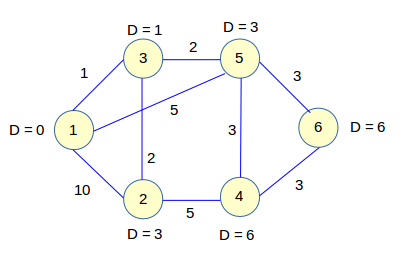
\includegraphics[width=0.4\textwidth]{./g6.png}
	\caption{Grafo ponderado 3}
	\label{fig:g6}
	\end{center}
	\end{figure}
	\end{itemize}
\end{itemize}

\subsection{Búsqueda con heurística}

Al igual que BFS, este algoritmo no tiene en cuenta los pesos, por lo que es ideal para grafos no ponderados o aquellos en los que todos los pesos son iguales. Para definir cual será el vertice que se analizará primero se definió una cola de prioridad que dependa de la distancia estimada por la heurística entre el vértice y el destino. En este caso, se usó como heurística el cálculo de la distancia Manhattan entre dos vertices, sobre grafos cuadrados, con el objetivo de poder compararlo con A*. Debido al uso de la cola de prioridad en el cual se agregan solo una vez todos los vértices, la complejidad será $O(|V| \log{|V|})$

\begin{itemize}
\item \textbf{Complejidad:} $O(|V| \log{|V|})$
\item \textbf{Mejores casos:}
	\begin{itemize}
	\item $O(|V| \log{|V|})$ si el grafo cumple la condición de ser cuadrado y no ponderado, o con todos sus pesos iguales. Ej:
	\begin{verbatim}
	origen = 0
	destino = 15
	\end{verbatim}
	\begin{figure}[H]
	\begin{center}
	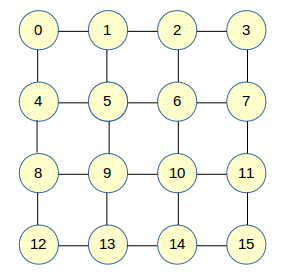
\includegraphics[width=0.3\textwidth]{./g7.png}
	\caption{Grafo no ponderado 2}
	\label{fig:g7}
	\end{center}
	\end{figure}
	\end{itemize}
\item \textbf{Peores casos:}
	\begin{itemize}
	\item $O(|A| \log{|V|})$ si la heurística no es buena y estima distancias erroneas. Esto puede pasar en caso de usar la distancia manhattan implementada sobre un grafo que no tenga la forma esperada. En el ejemplo, la arista roja, que pertenece al camino mínimo, tendrá peor prioridad en la cola que las demás, por lo que será necesario recorrer todo el grafo y puede que no devuelva el mejor camino. Ej:
	\begin{verbatim}
	origen = 0
	destino = 4
	\end{verbatim}
	\begin{figure}[H]
	\begin{center}
	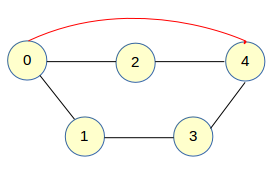
\includegraphics[width=0.3\textwidth]{./g8.png}
	\caption{Grafo no ponderado 3}
	\label{fig:g8}
	\end{center}
	\end{figure}
	\item En el caso de grafos ponderados, no se toma en cuenta el peso de las aristas, por lo que no se puede esperar el camino mínimo, sino solo uno de los existentes.
	\end{itemize}
\end{itemize}


\subsection{A*}

Para implementar $A*$ se usó la misma estructura que para la busqueda con heurística, solo que esta vez sí se tomó en cuenta el peso de las aristas en los grafos ponderados. Nuevamente, se usó la distancia Manhattan como heurística.

\begin{itemize}
\item \textbf{Complejidad:} $O(|V| \log{|V|})$
\item \textbf{Mejores casos:}
	\begin{itemize}
	\item $O(|V| \log{|V|})$ si el grafo cumple la condición de ser cuadrado y la heurística es buena, es decir no hay gran diferencia entre la distancia estimada y la real. Por ejemplo, en el grafo siguiente una heurística que priorice los vértices de menor valor que estén a una misma distancia del destino según Manhattan, será más efectiva que la distancia Manhattan pues el vértice 1 tendrá una prioridad mejor que el 4. Ej:
	\begin{verbatim}
	origen = 0
	destino = 15
	\end{verbatim}
	\begin{figure}[H]
	\begin{center}
	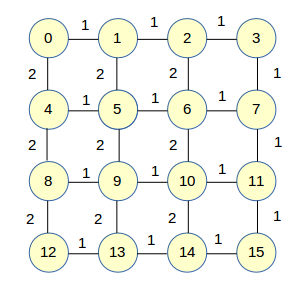
\includegraphics[width=0.3\textwidth]{./g10.png}
	\caption{Grafo ponderado 4}
	\label{fig:g10}
	\end{center}
	\end{figure}
	\end{itemize}
\item \textbf{Peores casos:}
	\begin{itemize}
	\item $O(|A| \log{|V|})$ si la heurística no es buena y estima distancias erroneas. Ej:
	\begin{verbatim}
	origen = 0
	destino = 4
	\end{verbatim}
	\begin{figure}[H]
	\begin{center}
	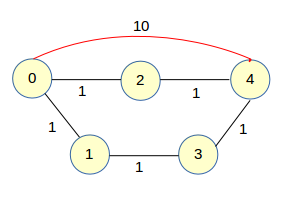
\includegraphics[width=0.3\textwidth]{./g9.png}
	\caption{Grafo ponderado 5}
	\label{fig:g9}
	\end{center}
	\end{figure}
	\end{itemize}
\end{itemize}


\subsection{Algoritmo con solución óptima}

A continuación se evalúan los resultados obtenidos para los grafos en las figuras anteriores*. Para cada uno se dirá si encontró la solución óptima y si es el más eficiente para ese caso. Para evaluar si es el más eficiente se compararon los tiempos de ejecución para cada uno de los algoritmos. Como heurística optimista se tomó una que siempre devuelva uno, que es el mínimo peso de una arista. Como pesimista se elegió una que devolviera siempre una distancia igual a la cantidad de vértices del grafo.

\subsubsection{Grafos no ponderados}

En algunos casos había varias soluciones óptimas, por lo cual se tomo como aceptable cualquiera de ellas.

\begin{table}[H]
\centering
\scalebox{0.7}{
\begin{tabular}{|c|c|c|c|c|c|c|}
\hline
\multirow{2}{*}{Algoritmo}	& \multicolumn{2}{c|}{Grafo Figura \ref{fig:g3}}	&\multicolumn{2}{c|}{Grafo Figura \ref{fig:g7}}	& \multicolumn{2}{c|}{Grafo Figura \ref{fig:g8}}\\
						&Óptima	&Más Eficiente	&Óptima	&Más Eficiente	&Óptima	&Más Eficiente\\\hline
BFS						& Sí	& Sí	& Sí	& No	& Sí	& No\\\hline
Dijkstra				& Sí	& No	& Sí	& No	& Sí	& No\\\hline
Heurística Manhattan	& Sí	& No	& Sí	& No	& Sí	& No\\\hline
Heurística Optimista	& Sí	& No	& Sí	& No	& Sí	& No\\\hline
Heurística Pesimista	& Sí	& No	& Sí	& No	& Sí	& No\\\hline
A* Manhattan			& Sí	& No	& Sí	& No	& Sí	& No\\\hline
A* Optimista			& Sí	& No	& Sí	& Sí	& Sí	& Sí\\\hline
A* Pesimista			& Sí	& No	& Sí	& No	& Sí	& No\\\hline
\end{tabular}
}
\caption{Resultados por grafo no ponderado}
\label{tab:datosexp}
\end{table}

Es evidente que para grafos no ponderados cualquier algoritmo devolvió la solución óptima. Sin embargo, los tiempos de ejecución variaron notablemente de unos a otros y dependiendo del grafo.

\subsubsection{Grafos ponderados}

\begin{table}[H]
\centering
\scalebox{0.5}{
\begin{tabular}{|c|c|c|c|c|c|c|c|c|c|c|}
\hline
\multirow{2}{*}{Algoritmo}	& \multicolumn{2}{c|}{Grafo Figura \ref{fig:g4}}	&\multicolumn{2}{c|}{Grafo Figura \ref{fig:g5}}	& \multicolumn{2}{c|}{Grafo Figura \ref{fig:g6}} &\multicolumn{2}{c|}{Grafo Figura \ref{fig:g10}}	& \multicolumn{2}{c|}{Grafo Figura \ref{fig:g9}}\\
						&Óptima	&Más Eficiente	&Óptima	&Más Eficiente	&Óptima	&Más Eficiente	&Óptima	&Más Eficiente	&Óptima	&Más Eficiente\\\hline
BFS						& No	& No			& Sí	& No			& No	& No			& Sí	& No			& No	& No\\\hline
Dijkstra				& Sí	& No			& Sí	& No			& Sí	& No			& Sí	& No			& Sí	& No\\\hline
Heurística Manhattan	& No	& No			& Sí	& No			& No	& No			& No	& No			& No	& No\\\hline
Heurística Optimista	& No	& No			& Sí	& No			& No	& No			& No	& No			& No	& No\\\hline
Heurística Pesimista	& No	& No			& Sí	& No			& No	& No			& No	& No			& No	& No\\\hline
A* Manhattan			& Sí	& Sí			& Sí	& Sí			& Sí	& No			& Sí	& Sí			& Sí	& No\\\hline
A* Optimista			& Sí	& No			& Sí	& No			& Sí	& No			& Sí	& No			& Sí	& No\\\hline
A* Pesimista			& Sí	& No			& Sí	& No			& Sí	& Sí			& Sí	& No			& Sí	& Sí\\\hline
\end{tabular}
}
\caption{Resultados por grafo ponderado}
\label{tab:datosexp}
\end{table}

Como se puede ver, para grafos ponderados la busqueda heurística y cualquier otro método, como BFS, que no tenga en cuenta los pesos no devolverá una solución óptima excepto algún caso particular. La heurística de la distancia Manhattan resultó ser mejor de lo esperado, aún con grafos que tenían formas distintas a la esperada.
\end{document}
